\chapter{Models}
\label{chap:models}
This section will expose the reader with the different model architecture used during the project. we decide not to go for a fancy deep learning algorithm such as ResNet\cite{resNet_he2015deep} for simplicity but it would be interesting to try them with more data to see the impact.

\section{Standard 3D CNN}
\label{sec:standard_cnn}

The model we choose for classification is composed of 12 convolutional layers each of size 3 by 3 by 3. The number of output channels gradually increase from 1 (gray-scale) to 32. As dealing with 3D images, one can not simply increase the number of channels as it would require a lot of GPU memory which is often a bottleneck. Therefore, we added a MaxPooling layer after every two Convolutional layer. This technique is used to reduce the image size, but this is not the only way of reducing the image size. In fact when performing standard convolution with a kernel of size k. The output shape in each dimension will be of $s_{out} = \frac{s_{in} - k + 2* pad}{stride} + 1$, where $k$ is the kernel size, $pad$ the added padding and $s_{in}$ the input size. In this work we focused on building a model that we could explain its prediction as much as possible. For some reason that we realized, it was important to keep the shape of the image unchanged after each convolution layer, otherwise we got some alignement issue between the image and the saliency map once interpolated to the image dimensions. The image is therefore padded with zeros all around in order to prevent it from this artifacts. Between every layer, we choose to activate the layer output with the classical Relu\cite{relu_10.5555/3104322.3104425} function. The main reason behind this choice, is the need for easy interpretability with the FullGrad algorithm (current implementation only support the relu activation function).  
The convolutional layers are good for extracting relevant features for the task. Those features are then fed into a classifier composed of two linear layers. A dropout\cite{dropout_10.5555/2627435.2670313} layer has been added in between those layers in order to reduce overfitting.

\section{3D CNN with Global Average Pooling}

The model described above has quite a lot of parameters to learn especially due to the last linear layers. In fact when flattening the reduced image it can become a big vector. This has the disadvantages of being harder to train and demands a larger amount of training data. As already stated at the time of writing we do not have a lot of data to train our model. 
To overcome that we slightly changed the design of our network and replaced the flattening layer by a \textit{Global Average Pooling Layer}\cite{GAP_lin2013network} (GAP). This changed dramatically reduced the size of the classifier which allowed us in consequence to increase the number of output channels of our features extractor to 128.  
This technique is often performed in computer vision and has the advantage of allowing the network to infer on data of almost any size. By construction it gives the network a translation invariance property in the opposite of being only equivariant to translation for standar 3D CNN.
With regards to our preprocessing this might in fact be a feature not well suited, as all the brain scans are registered into the same space meaning that a specific pixel is gonna encode a specific location inside the brain. This global average pooling has in fact the disadvantage of losing some spatiale location property. 


\section{Unbias model}
\label{sec:unbias_model}

Often the data you are working with present an underlying bias. For example in the case of Alzheimer disease, it appears that old people are more likely to be diagnosed with the disease than young ones (see figure \ref{fig:OASIS_age_dist}). As this might be debatable whether or not age should be taken into account in order to predict dementia. Experiments on age prediction in annex \ref{chap:age_pred}, shows that age is an hidden feature well present in MRI scan.

\begin{wrapfigure}{r}{0.6\textwidth}
 \centering
 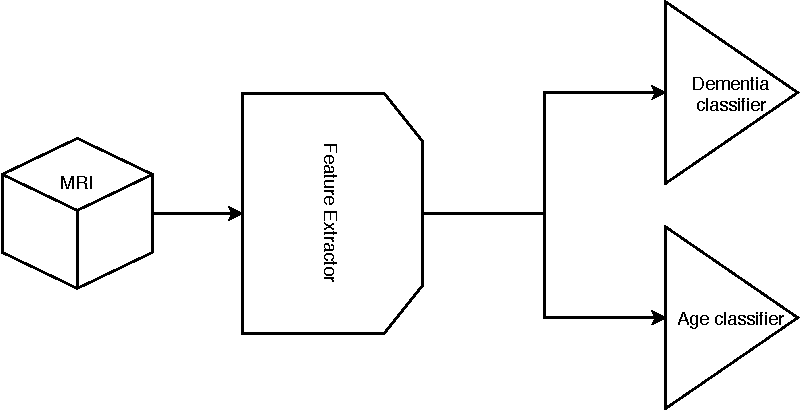
\includegraphics[width=.9\linewidth]{figures/models/Unbias_model.pdf}
 \captionsetup{width=.9\linewidth}
 \caption[UnbiasModelSchema]{Unbias Model Schema.}
 \label{fig:unbias_model_schema}
\end{wrapfigure}

Such bias can of course fool the model, that might be overconfident on classifying old people as dement or even worst young people as healthy just because in the training set dement sample were mostly old people.
Note that by building the model below we are indeed only interested in mitigating the bias due to age, but this model can be easily modified in order to mitigate other potential bias as long as you have a label for the bias you want to mitigate. Example of other bias might be sex, left or right handed, or even the hosiptal/machine used for scanning


As illustrated by figure \ref{fig:unbias_model_schema}, the model is composed of 3 elements. The \textit{feature extractor} extract a fix amount of features from the MRI using convolutional layers in a similar manner as the other models describe in chapter \ref{chap:models}. The \textit{dementia classifier} and \textit{age predictor}, are both composed of fully connected layer, with 1 feature as output. The dementia classifier has a sigmoid function on top of it as its task is a binary classification while the age predictor does not have an activation function on its output.

What makes this model interesting it the way we train it. For that we need two optimizer, one that works on the weights of the feature extractor and the weights of the age classifier. While the other works with on the weights of the age predictor only. In addition to the classic dementia loss (BCE) and the age predictor one (MSE), we define a new loss $L_{3}$ to be: $L_3 = L_{dementia} - \lambda L_{age}$. The final goal is a Min-Max game where the first optimizer tries to minimize the $L_3$ loss while the second one tries to minimize the $L_age$ one. This model is inspire by the GAN\cite{goodfellow2014generative} architecture and requires a lot of fine tuning to get a stable training.  